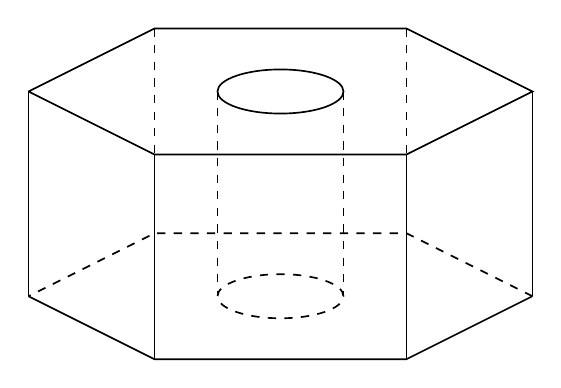
\begin{tikzpicture}[line width=0.6pt, font=\normalsize]
% Hexagonal prism block with central cylindrical through hole
% top hexagon (fully visible)
\coordinate (T1) at (-3.2,1.4);
\coordinate (T2) at (-1.6,2.2);
\coordinate (T3) at (1.6,2.2);
\coordinate (T4) at (3.2,1.4);
\coordinate (T5) at (1.6,0.6);
\coordinate (T6) at (-1.6,0.6);
% bottom hexagon (front visible, back hidden)
\coordinate (B1) at (-3.2,-1.2);
\coordinate (B2) at (-1.6,-0.4);
\coordinate (B3) at (1.6,-0.4);
\coordinate (B4) at (3.2,-1.2);
\coordinate (B5) at (1.6,-2);
\coordinate (B6) at (-1.6,-2);
% prism top outline
\draw (T1) -- (T2) -- (T3) -- (T4) -- (T5) -- (T6) -- (T1);
% front / side verticals solid
\draw (T1) -- (B1);
\draw (T6) -- (B6);
\draw (T5) -- (B5);
% back verticals dashed
\draw[dashed] (T2) -- (B2);
\draw[dashed] (T3) -- (B3);
\draw (T4) -- (B4);
% bottom front solid, back dashed
\draw (B1) -- (B6) -- (B5) -- (B4);
\draw[dashed] (B4) -- (B3) -- (B2) -- (B1);

% cylinder hole: top rim full ellipse, walls dashed, bottom rim dashed
\draw (0,1.4) ellipse (0.8 and 0.28);
\draw[dashed] (-0.8,1.4) -- (-0.8,-1.2);
\draw[dashed] (0.8,1.4) -- (0.8,-1.2);
\draw[dashed] (0,-1.2) ellipse (0.8 and 0.28);
\end{tikzpicture}
